\chapter{Problem statement and background}
\label{kap:problem}

In this chapter, we shall define what kind of problem we want to solve, so we better understand why it is interesting to work on such a task, and also specify the terminology and methods that we will use throughout this thesis.

\section{Our goal}
Defining properties of materials in the scene is essential for matching appearance of real world materials, but it is time consuming. This procedure can be dramatically simplified, as artists and graphic designers create new looks from already existing artworks. If they were able to transfer material characteristics from an image of these designs, it would be a time saver. Our goal is therefore to offer them a tool that would determine the most used material attributes from a single image.
\newline
To accomplish this goal, we need to perform per-pixel material segmentation, and then for this segmented material approximate selected scene or material characteristics. This approximation can be achieved by doing inverse rendering of a scene.
\newline
As we will show in chapter \ref{kap:prior}, there has been a lot of research lately regarding inverse rendering. Using deep learning techniques to tackle problems from different areas of interest proved to be very successful, so it was naturally applied to the computer vision field, and in our case, to inverse rendering as well. We believe that combination of these approaches will enable us to solve our task successfully.
\newline
As this work requires knowledge of terminology, methods and concepts from both computer graphics and machine learning, we elucidate both of these areas in the next sections.

\section{Terminology and methods in rendering}
    \subsection{Rendering}
    Rendering is a major subfield of the computer graphics area. Rendering is a sequence of steps to produce a 2D image from 3D representation of a scene stored in a computer. During this sequence -- which is also called the rendering pipeline -- the algorithm for handling rendering of a scene needs to take model representations, apply transformations, illuminate the scene from all lights presented, map textures to objects, throw away parts of the scene which will not be rendered, and finally draw an image from the camera view. There are several types of renderings based on different rendering algorithms, mostly divided into two categories: non-photorealistic rendering and photorealistic rendering, sometimes also called physically based rendering (PBR). The latter implements the concepts of transport and scattering of light in the real world, which is far more computationally expensive than the former approach but produces more plausible results. To look real when rendered, PBR needs (among other parameters) to have correctly set up material model, usually referred to as BRDF.
    \subsection{Bidirectional Reflectance Distribution Function}
    Bidirectional Reflectance Distribution Function (or BRDF for short) is a probabilistic function $f_r(\omega_i, \omega_o) \; (f_r(\omega_i \to \omega_o))$ describing how light is reflected based on surface attributes. More specifically, given incoming light direction $\omega_i$ and outgoing direction $\omega_o$, it gives the probability that a photon arriving from direction $\omega_i$ will be reflected to direction $\omega_o$.
    \newline
    There are several categories of BRDF models, of which the most impactful ones are the physically based BRDFs. To consider a BRDF model to be physically based, it must meet the following properties:
    \begin{itemize}
        \item positivity: $f_r(\omega_i, \omega_o) \geq 0$
        \item obeying Helmholtz reciprocity: $f_r(\omega_i,\omega_o) = f_r(\omega_o, \omega_i)$
        \item conserving energy: $\int_{\Omega} f_r(\omega_i, \omega_o) \cos \theta_i \; d\omega_i \leq 1 \;\; \forall \omega_o$
    \end{itemize}
    where $\cos \theta_i$ represent decrease of radiance with increasing $\theta_i$ (angle between $\omega_i$ and surface normal).
    \newline
    To achieve realistic material look, it is important to use such BRDF that satisfies these properties. Example of such BRDF can be physically based Phong BRDF, which is equal to
    \begin{equation}
        f^{Phong}_r = \frac{\rho_d}{\pi} + \frac{\rho_s(n + 2)\cos^n \theta_r}{2\pi}
        \label{eq:phong_correct}
    \end{equation}
    where $\rho_d$ stands for diffuse albedo, $\rho_s$ for specular albedo, $n$ for glossiness and $\theta_r$ for angle between view vector and reflected light vector.
    \subsection{Reflection equation}
    Knowing the BRDF of a surface allows us to compute how much light coming from direction $\omega_i$ is reflected from the surface to direction $\omega_o$. For that one has to multiply radiance $L_i$ from direction $\omega_i$, BRDF $f_r(w_i \to w_o)$ and $\cos \theta_i$. Summarized in mathema-tical notation:
    \begin{equation}
        L_r(\omega_i \to \omega_o) = L_i(\omega_i) \cdot f_r(\omega_i \to \omega_o) \cdot \cos \theta_i
    \end{equation}
    \newline
    In order to compute the total radiance reflected to direction $\omega_o$ we need to sum up the contributions from all light sources, direct or indirect. This can be done by integrating these contributions over upper neuron hemisphere $H(x)$, which gives us the following equation
    \begin{equation}
    \label{eq:reflection-equation}
        L_r(\omega_o) = \int_{H(x)} L_i(\omega_i) \cdot f_r(\omega_i \to \omega_o) \cdot \cos \theta_i \; d\omega_i
    \end{equation}
    also called reflection equation. This integral generally does not have an analytical solution and has to be computed numerically.
    \subsection{Monte Carlo integration}
    A typically used numerical method for solving integrals in rendering is Monte Carlo integration. This technique uses random numbers to sample points at which the integrand is evaluated. Let's denote an integral that we want to approximate, as
    \begin{equation}
        I = \int g(x) dx
    \end{equation}
    Monte Carlo estimation of $I$ is defined as
    \begin{equation}
        \label{eq:monte-carlo}
        \langle I \rangle = \frac{1}{N}\sum_{k = 1}^N \frac{g(X_k)}{p(X_k)},
    \end{equation}
    where $N$ is the number of samples taken, $X_k$, $k=1,...,N$ are the samples and $p(x)$ is a probability density function from which the samples were drawn.
    \newline
    By substituting equation \ref{eq:reflection-equation} into equation \ref{eq:monte-carlo}, the result is
    \begin{equation}
         \langle L_r(\omega_o) \rangle = \frac{2\pi}{N} \sum_{k = 1}^N L_i(\omega_{i, k})f_r(\omega_{i, k} \to \omega_o) \cos \theta_{i, k}
         \label{eq:monte-carlo-rendering}
    \end{equation}
    where $2\pi$ stands for the probability density function ($p(X_k) = \frac{1}{2\pi}$) of uniform sampling directions on the hemisphere and $\omega_{i, k}$, $k=1,...,N$ are the sampled directions.
    \newline
    An image can be rendered by evaluating equation \ref{eq:monte-carlo-rendering} for each of its pixels. Given such an image, our goal is to estimate what material (i.e.\ $f_r(\omega_{i, k} \to \omega_o)$) was used when the image was rendered. 
    \subsection{Inverse rendering}
    One of the possible methods for estimating what materials are present in an image is inverse rendering. Inverse rendering is one of the principal and long-standing problems in computer vision and computer graphics. Its main goal is to, provided an image or several images of a scene, estimate intrinsic properties of a scene, like depth, albedo, normals, reflectance, lighting and so on. This problem is hard for several reasons, mainly, as stated in \cite{li-inverse-rendering}: \glqq{}This is an ill-posed task: these scene factors interact in complex ways to form images and multiple combinations of these factors may produce the same image.\grqq{} As we can see, there is an infinite number of solutions for parameters for a single image, which makes the problem hard or almost impossible to solve. However, some solutions are statistically more admissible than others. Citing \cite{BarronTPAMI2015}, which says: \glqq{}Our goal is therefore to recover the most likely explanation that explains an input image.\grqq{} To make this work, we need to come up with such statistics that would correctly approximate the real world. This is not straightforward, but recent advances in both optimization and learning based approaches show that it's possible to estimate a handful of properties correctly \cite{BarronTPAMI2015} and even better results when physically based datasets were used for training neural networks \cite{sengupta-inverse-rendering}\cite{li-inverse-rendering}. With these properties in hand, we want to estimate what is the material on the user-specified object in the image.
    \begin{figure}[H]
        \centerline{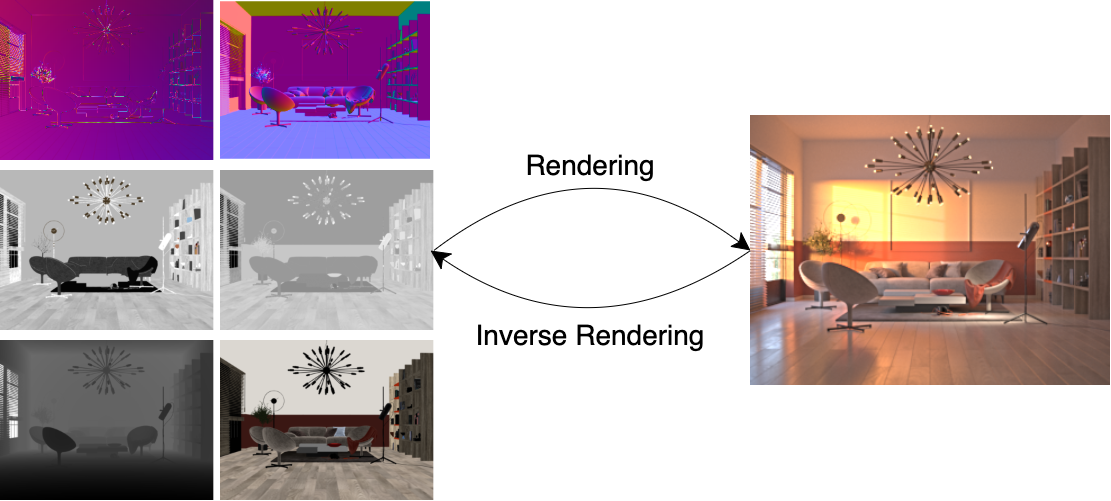
\includegraphics[width=0.6\textwidth]{praca/images/Rendering vs Inverse Rendering.png}}
        \caption[Rendering vs inverse rendering]{Rendering vs inverse rendering}
        \label{img:rendering-vs-inverse-rendering}
    \end{figure}
\section{Terminology and methods in machine learning}
    \subsection{Machine learning}
    For quite some time, mathematicians wondered if it's possible to create thinking machines. The solution to this idea was to allow computers to learn complex concepts from simple ones or experience. We provide this experience in the form of a dataset, which consists of information (usually called features) about the task that we want to train the model for. Generally, we let the algorithm decide which features are important and how will individual features contribute to its final prediction. We call this ability of computers as machine learning. Machine learning is an outstandingly fast advancing area of research, and it helps to push research forward in other areas as well. Computer graphics is not an exception as machine learning techniques are used in calculating direct illumination \cite{Vevoda-rendering} for example.
    \subsection{Neural networks}
    Human brains consist of nerve cells, which are called neurons. These neurons form large networks where they can propagate information from one neuron to the other. The purpose of neural networks (NNs) as a machine learning method is to mimic these networks to be able to learn and make decisions. The main difference between neural networks and traditional programming is that while in traditional programming we explicitly instruct a computer what to do in each step of the program, we don't instruct neural networks how to behave or how to solve the task. We simply allow it to examine the provided data and let it propose a solution. This solution can be viewed as mapping $\mathcal{F'}$, where $\mathcal{F}$ is the underlying mapping that we want to approximate. $\mathcal{F'}$ should be optimal in some sense - we need such $\mathcal{F'}$ that minimizes $$\frac{\sum_{x \in X} error(\mathcal{F}(x) - \mathcal{F'}(x))}{|X|}$$ where $X$ is a set of inputs to the neural network.
    \newline
    Neural network consists of several layers, which are called input, hidden and output layer, with input and output layers required in every neural network, but any non-negative number of hidden layers is allowed. Every layer consists of several neurons. In the most common type of neural network, all neurons from previous layer are connected with all neurons in the next layer. These connections are called \textbf{weights} and network learns them throughout the training. We can see weights between one layer to other in figure \ref{fig:neural_network} and an example of a simple neural network in figure \ref{img:simple_nn}.
    \begin{figure}
        \centering
        \tikzset{%
          every neuron/.style={
            circle,
            draw,
            minimum size=0.5cm
          },
          neuron missing/.style={
            draw=none, 
            scale=4,
            text height=0.15cm,
            execute at begin node=\color{black}$\vdots$
          },
        }
        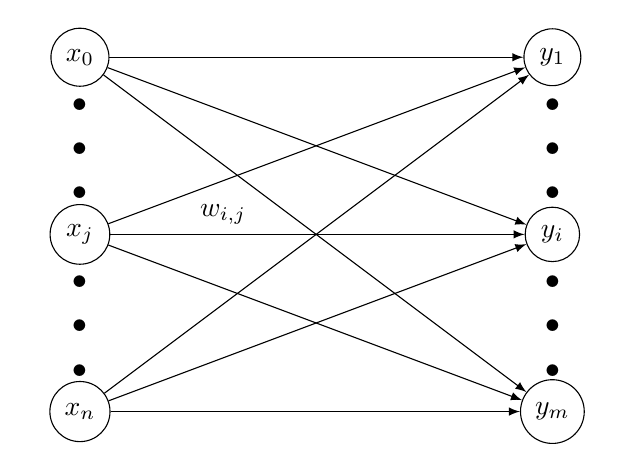
\begin{tikzpicture}[x=1.5cm, y=1.5cm, >=stealth]
        \node [every neuron] (input-1) at (-2,1) {$x_0$};
        \node [neuron missing] (input-missing-1) at (-2, 0) {};
        \node [every neuron] (input-j) at (-2,-0.5) {$x_j$};
        \node [neuron missing] (input-missing-2) at (-2, -1.5) {};
        \node [every neuron] (input-n) at (-2,-2) {$x_n$};
        
        \node [every neuron] (output-1) at (2,1) {$y_1$};
        \node [neuron missing] (output-missing-1) at (2, 0) {};
        \node [every neuron] (output-i) at (2,-0.5) {$y_i$};
        \node [neuron missing] (output-missing-2) at (2, -1.5) {};
        \node [every neuron] (output-m) at (2,-2) {$y_m$};
        
        \path [draw, -latex] (input-1) -- (output-1);
        \path [draw, -latex] (input-1) -- (output-i);
        \path [draw, -latex] (input-1) -- (output-m);
        
        \path [draw, -latex] (input-j) -- (output-1);
        \path [draw, -latex] (input-j) -- node[left=1.2cm, midway, above] {$w_{i, j}$} (output-i);
        \path [draw, -latex] (input-j) -- (output-m);
        
        \path [draw, -latex] (input-n) -- (output-1);
        \path [draw, -latex] (input-n) -- (output-i);
        \path [draw, -latex] (input-n) -- (output-m);
        
        \end{tikzpicture}
        \caption[Connections between two layers of neural network]{Connections between two layers of neural network, circles are neurons and lines represent weights, weight $w_{i, j}$ represents connection between neuron $j$ in first layer and neuron $i$ in second layer}
        \label{fig:neural_network}
    \end{figure}
    Neural network performs two operations -- \textbf{forward propagation and back-propagation}. The former is used to get the prediction, the latter to adjust weights in the system to account for the computed error. During forward propagation, neural network computes values for all neurons in the next layer based on the previous layer. These values are then fed through some non-linearity function $f$ to keep all the values in certain range (for example between $0 \leq x \leq 1$ or $-1 \leq x \leq 1$). Computed values are called \textbf{activations} of neurons. This process repeats until the network compute values in output layer. Equation \ref{eq:feed-forward} summarizes the process of computing activation of one neuron, where $n$ and $m$ are the number of neurons in first layer and second layer respectively. Common thing to help neural network learn better is to add a \textbf{bias term} to the layer and set it as $x_0 = 1$.
    \begin{equation} \label{eq:feed-forward}
        y_i = f(\sum_{j=0}^{n} w_{i, j} * x_j) \; \; \; \; \forall i \in \{1, \dots, m \}
    \end{equation}{}
    \begin{figure}
        \centerline{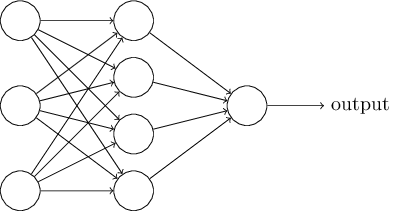
\includegraphics[width=0.4\textwidth]{praca/images/nn.png}}
        \caption[Example of a simple neural network]{Example of a simple neural network with input, hidden and output layer. Circles represent neurons, lines between neurons show connections from neuron in one layer to neuron in the next layer. Taken from \cite{nielsenneural}.}
        \label{img:simple_nn}
    \end{figure}
    \newline
    When we have computed the prediction, we need to adjust weights in a network to account for the difference between predicted value and the actual value. The error is then propagated back through the network in order to compute gradient, which is in turn used by some optimization method (for example gradient descent) to find local minimum of an error function, which is a metric for evaluating network's performance. The process of forward and back-propagation is repeated many times for every entry in the dataset until convergence.
    \subsection{Deep learning and deep neural networks} \label{deep-learning}
    Deep learning is a special kind of machine learning which is capable to learn more complex functions than simpler methods of machine learning. Every neural network that has more than one hidden layer can be considered a deep neural network. These multiple layers help the network to develop several levels of abstraction, which can give deep networks an upper hand in recognizing complex patterns over other methods or models \cite{deep-learning}. This is why so many solutions to pattern recognition problems employ this technique, but because of the relatively high computation power required for it's training, it wasn't used until very recently. Most models for inverse rendering use deep convolutional neural networks, which we will define in the next section.
    \subsection{Convolutional neural networks}
    Convolutional neural networks (CNNs, or sometimes just convolutional networks), are neural networks that are specially designed to process grid-like structured data, like images or videos.
    \newline
    Neural networks use matrix multiplication and activation function to compute the activation of neurons in the next layer. CNNs on the other hand, use a different approach - at least in one of their layers, they use a special kind of linear operation called convolution, which is defined as 
    $$ s(t) = \int x(a) * w(t - a) \mathrm{d}a $$
    with $x$ is often referred to as the input and function $w$ as the kernel. The output of the convolution is referred to as the feature map(s). Convolutional layers convolve the input with the help of the kernel function -- which is just a function that transforms original input space into space, where it can be easier to train the model due to change from non-linear to a linear problem -- and pass its result to the next layer. This is similar to the response of a neuron in our brain to a specific impulse. Because of this property, CNN is a great model for extracting edge information from images. Convolution layer in CNNs consists of convolution stage, detector stage and pooling stage. During convolution stage, several convolutions are run in parallel to produce many layers of linear activations. During detector stage, all of these layers are run through some non-linear function to produce activations in certain range. And finally, during pooling stage, we use pooling function to produce statistical analysis of a specific neighbourhood in every layer. Typical CNN architecture for digit recognition can be seen in figure \ref{fig:cnn}.
    \begin{figure}
        \centerline{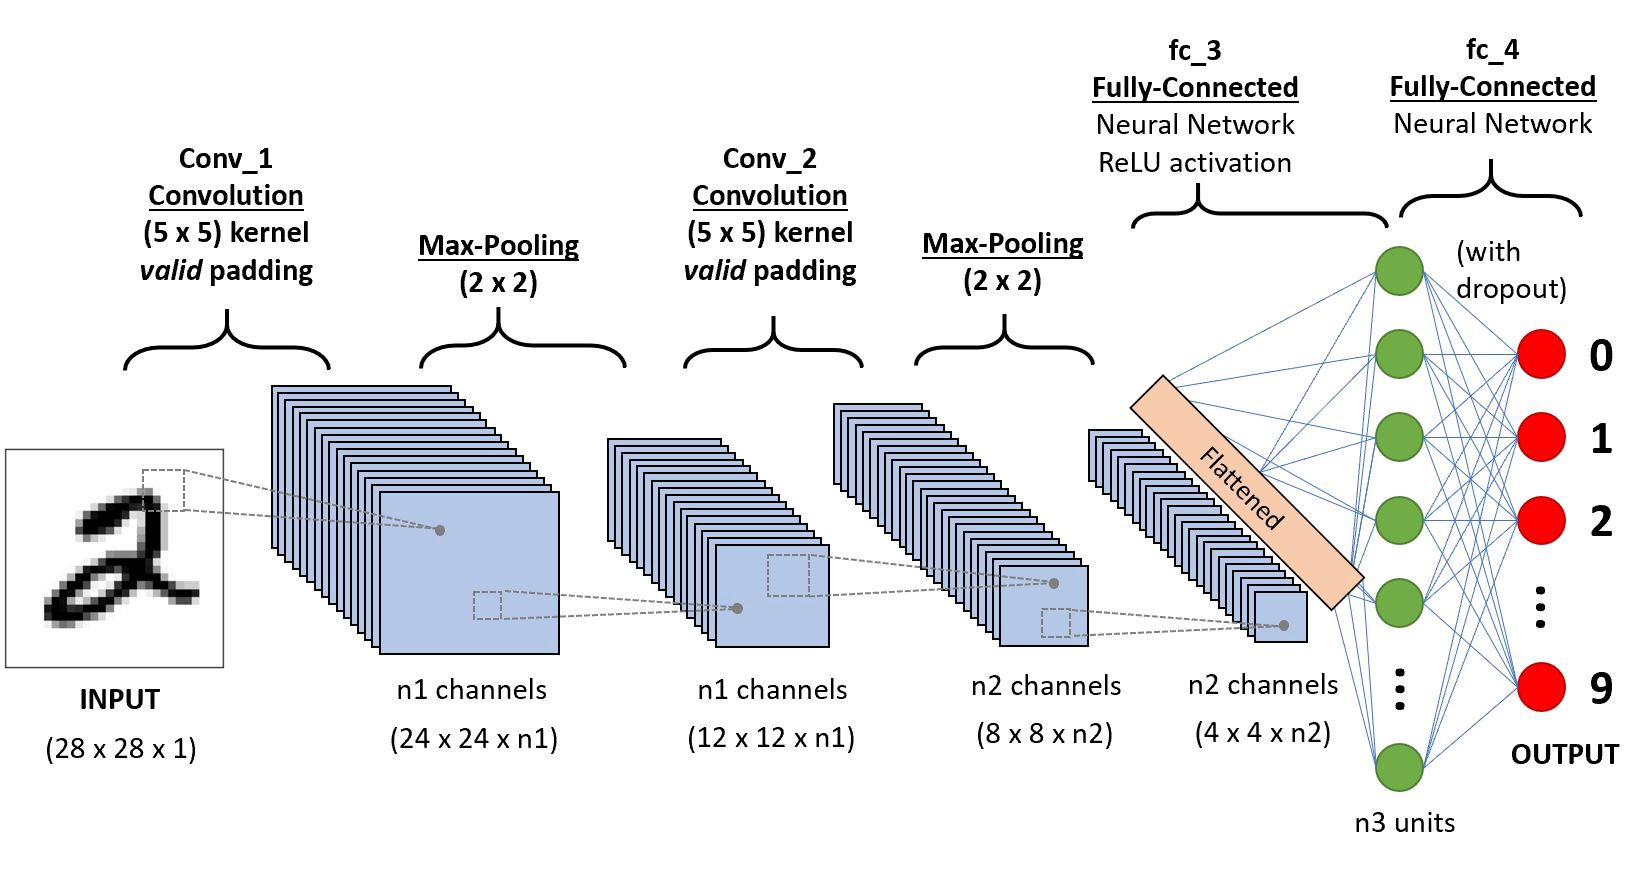
\includegraphics[width=0.7\textwidth]{praca/images/cnn_architecture.jpeg}}
        \caption[Typical CNN architecture for digit recognition]{Typical CNN architecture for digit recognition, taken from \cite{cnn}. The original image is run through several convolutional layers before finally being flattened with digit predictions as output}
        \label{fig:cnn}
    \end{figure}
    \newline
    Another important property of CNN is its effectiveness when compared to traditional neural networks - performing convolution in layers of CNN is faster and requires orders of magnitude less storage then using NN for the same kind of problem \cite{deep-learning}. As a result, CNNs perform tremendously on image recognition tasks and are now one of the state-of-the-art solutions for this challenging problem.
    \subsection{Residual neural network}
    As we stated in section \ref{deep-learning}, deep networks have the ability to learn several layers of abstraction, which means that depth is important. This is especially valuable when working with images or videos, as these layers can help decompose input image into low to high level features of the image. However, just adding more and more layers brings problems like non-convergence of the whole network or 
    accuracy degradation. The former was mostly resolved by normalized initialization, the latter by introduction of residual learning, with residual neural network as its architecture \cite{residual-network}. Residual neural network is network consisting of residual blocks, as shown in figure \ref{fig:res_block}.
    \begin{figure}
        \centerline{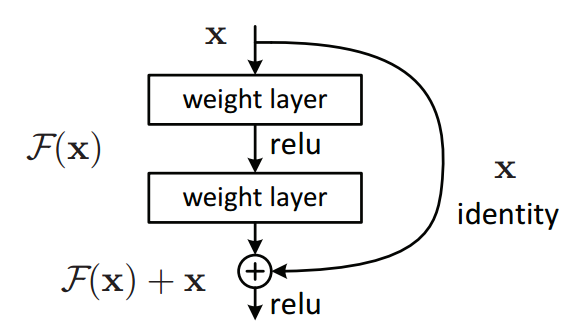
\includegraphics[width=0.4\textwidth]{praca/images/residual-block.png}}
        \caption[Example of residual block]{Example of residual block}
        \label{fig:res_block}
    \end{figure}
    Idea behind this block architecture is that rather than finding mapping $\mathcal{H}(x)$ that would be optimal for this block without any prior, we reformulate the mapping that the block should learn to $\mathcal{F}(x) = \mathcal{H}(x) - x$, so the output mapping then becomes $\mathcal{F}(x) + x = \mathcal{H}(x)$. This helps with training particularly where output of the block should be very similar to its input, like in cases where identity mapping is the optimal mapping. We use residual blocks in our networks a lot because they enable us to train deeper models, as they are easier to optimize than conventional CNN networks \cite{residual-network}.